% !TEX encoding = UTF-8 Unicode
\documentclass[a4paper]{article}

\usepackage{color}
\usepackage{url}
\usepackage{graphicx}

\usepackage[english,serbian]{babel}

\usepackage[unicode]{hyperref}
\hypersetup{colorlinks,citecolor=green,filecolor=green,linkcolor=blue,urlcolor=blue}

\newtheorem{primer}{Primer}[section]

\usepackage[bottom]{footmisc}
\usepackage[linesnumbered,ruled]{algorithm2e}

\usepackage{type1ec}
\usepackage{cmap}
\defaulthyphenchar=127

\newcommand{\dvareda}[2][c]{\begin{tabular}[#1]{@{}c@{}}#2\end{tabular}}
\newcommand{\autori}[8]{\author{\begin{tabular}{c c} \dvareda{#1\\#2} & \dvareda{#3\\#4}\\\dvareda{#5\\#6} & \dvareda{#7\\#8} \end{tabular}}}

\newenvironment{algoritam}[1][htb]
{\renewcommand{\algorithmcfname}{Algoritam}
\begin{figure}[ht]
\centering
  \begin{minipage}{.75\linewidth}
	\begin{algorithm}[#1]%
  }{\end{algorithm}
  \end{minipage}
\end{figure}}

\providecommand{\keywords}[1]
{
	\small	
	\textbf{\textit{Ključne reči ---}} #1
}

\begin{document}

\title{Paralelizacija metaheuristika\\ \small{Seminarski rad u okviru kursa\\Metodologija stručnog i naučnog rada\\ Matematički fakultet}}

\autori{Jovan Mirkov}{jvnmirkov@gmail.com}{Lazar Vasović}{lazar1997@mts.rs}{Dušica Golubović}{dusica.golubovic@yahoo.com}{Teodora Heldrih}{heldrich013@gmail.com}

\maketitle

\abstract{Ukratko su opisani zadaci matematičke optimizacije i njihova moguća rešenja na primeru problema trgovačkog putnika, kao i problemi koji se susreću pri svakom od pristupa. Uz razvoj novih tehnologija rastu i mogućnosti današnjih računara, ali i potreba za bržim usavršavanjem. Kao rešenje nedovoljne brzine izvršavanja metaheuristika, predloženo je njihovo unapređenje paralelizacijom. Uz opširnu motivaciju, izloženo je nekoliko različitih modela u zavisnosti od potreba i tipa približnog metoda koji se paralelizuje. Uz svaki tip izložen je po jedan ilustrativan primer problema.}

\keywords{optimizacija, metaheuristike, paralelizam}

\tableofcontents

\newpage

\section{Uvod}
\label{sec:uvod}
Veliki udeo realnih problema u računarstvu i drugim sferama života koji se rešavaju tehnikama optimizacije jeste NP-težak, ili na neki drugi način komplikovan za tačno rešavanje. Kao dobro rešenje pokazale su se metaheuristike. One se danas koriste u raznim oblastima: optimizaciji, bioinformatici, razvoju softvera, pa sve do telekomunikacija i ekonomije \cite{alba, alba2}. Više o optimizacionim problemima, metaheuristikama i zašto i kako je moguće ubrzati metaheuristike paralelizacijom, opisano je u poglavlju \ref{sec:optimizacioniProblemi}.
U poglavlju \ref{sec:ParalelneMetaheuristike} opisana je podela metaheuristika na metaheuristike zasnovane na populaciji i metaheuristike zasnovane na unapređenju jednog rešenja. Prvo je opisan algoritam metaheuristike zasnovane na populaciji (poglavlje \ref{sec:OsnovnoPopulacija}) i njegova primena na paralelizaciju algoritama evolucije (poglavlje \ref{sec:ParalelizacijaEvolucije}), kao i konkretna primena na paralelizaciju genetskog algoritma u okviru istog podnaslova. Paralelizacija metaheuristike zasnovane na unapređenju jednog rešenja je opisana u poglavlju \ref{sec:ParalelizacijaJednog}.

\section{Optimizacioni problemi i rešenja}
\label{sec:optimizacioniProblemi}

\textbf{Matematička optimizacija}, poznata i kao \textbf{matematičko programiranje}, predstavlja odabir najboljeg elementa iz nekog skupa potencijalnih rešenja proučavanog problema prema određenom kriterijumu. Kako se odabir vrši pretraživanjem skupa rešenja, optimizacioni algoritmi spadaju u algoritme pretrage. Kriterijum pretrage najčešće je iskazan ciljnom funkcijom koju treba minimizovati ili maksimizovati (ova dva problema su ekvivalentna, pošto se maksimizacija funkcije $f$ svodi na minimizaciju $-f$), a opciono i skupom ograničenja koji mora biti zadovoljen kako bi rešenje bilo prihvatljivo, odnosno dopustivo, pošto su kod izrazito teških problema ponekad prihvatljiva i relativno dobra nedopustiva rešenja, koja samo u maloj meri ne ispunjavaju neko od nametnutih ograničenja.

\subsection{Pristupi rešavanju}

Za potrebe daljeg teksta, uvodi se sledeći motivacioni primer.

\begin{primer}
Neka je zadat skup $G$ od $n$ gradova i funkcija udaljenosti $d(g_i, g_j)$ za svaki par gradova. Pronaći permutaciju $p: [1..n] \mapsto [1..n]$ takvu da je ukupna suma udaljenosti grana koje se prolaze obilaskom minimalna.
\end{primer}

Naveden je \textbf{problem trgovačkog putnika} (eng. \textit{travelling salesman problem}, TSP), jedan od najpoznatijih problema kombinatorne optimizacije. Verzija sa odlučivošću -- postoji li put (permutacija) dužine manje od zadatog $L$  -- poznata je u teoriji složenosti kao jedan od prototipnih NP-kompletnih problema, što znači da je poznat način rešavanja isključivo u eksponencijalnom vremenu. To nadalje znači da najverovatnije nije moguće sa sigurnošću odrediti traženu permutaciju kod osnovnog problema bez provere svih $n!$ mogućnosti \cite{ri}.

Ovakav raspored činilaca navodi na zaključak da je \textbf{egzaktno} rešavanje ovog i sličnih problema neisplativo. Već za dvadesetak gradova, metod grube sile poput totalne enumeracije morao bi da proveri preko dva triliona ($20! > 2\cdot10^{18}$) potencijalnih rešenja, pri čemu bi evaluacija svakog sabirala desetine grana. Iz tog razloga se, u slučaju da nije od prevelike važnosti dobijanje tačnog rešenja, pribegava upotrebi \textbf{heuristika}. One daju približno rešenje, ali se izvršavaju u polinomskom vremenu. Uprkos efikasnosti dobijanja, heuristička rešenja mogu biti problematična zbog lošeg kvaliteta, tako da se često primenjuju heuristike sa određenom garancijom kvaliteta. Primera radi, za slučaj TSP u euklidskoj ravni (važi i za druge mere sa svojstvom nejednakosti trougla) osmišljena je 2-aproksimativna heuristika \cite{ri} koja dokazano pronalazi rešenje koje je u najgorem slučaju dvaput lošije (duže) od optimalnog, i to u kvadratnom vremenu \cite{aa}.

Problem mnogih heuristika jeste njihova specifičnost. Jednom osmišljena heuristika, poput 2-aproksimativne za TSP, često nije ponovo upotrebljiva, osim za neke veoma slične probleme. Stoga se za potrebe naglašavanja upotrebljivosti na širokom spektru optimizacionih problema uvodi pojam \textbf{metaheuristike}. Metaheurističke metode opisuju opšte strategije pretrage za rešavanje optimizacionih problema \cite{vi}. Formulisane su nezavisno od konkretnog problema, ali najčešće su prilično parametrizovane, pa ih je pre pokretanja moguće prilagoditi posebnom problemu koji se rešava. Poput drugih približnih metoda, metaheuristike razmatraju samo mali deo skupa mogućih rešenja, ali s druge strane uglavnom ne daju nikakve garancije o kvalitetu dobijenog rešenja. Ipak, rezultati su često dovoljno dobri i prihvatljivi, posebno u situacijama kada bi jedina alternativa bila egzaktna metoda koja bi se izvršavala neprihvatljivo dugo.

\subsection{Može li bolje?}

Uprkos tome što se približnim rešavanjem znatno poboljšava vremenska složenost pretrage, često ni dužina izvršavanja metaheuristike nije zadovoljavajuća. Uobičajene metaheuristike uglavnom su sekvencijalne -- svaki deo algoritma izvršava se jedan za drugim. Kako to često nije nužno, kao dobar način unapređenja javlja se \textbf{paralelizacija}. Uopšteno se pod ovim pojmom podrazumeva pisanje ili prilagođavanje programa tako da koriste mogućnosti paralelnog izvršavanja \cite{rs}. Konkretno, ukoliko je raspoloživo više izvršnih jedinica u vidu procesora ili jezgara, moguće je istovremeno izvršavati pojedine delove metaheurističkih algoritama. Prema tipu podele posla između jedinica, moguće je:

\begin{itemize}
\item \textbf{paralelizovati zadatke} -- npr. jedna nit pokreće glavni program dok druge računaju neke međukorake (konkurentnost na nivou jedinice),
\item \textbf{paralelizovati podatke} -- npr. svako rešenje se obrađuje i ažurira na posebnoj niti (\textit{paralelizacija petlji}, konkurentnost na nivou naredbe).
\end{itemize}

Iz prethodne podele nazire se i drugi razlog paralelizacije, pored dobijanja na performansama. U pitanju je podela posla, odnosno razdvajanje odgovornosti, odnosno podrška logičkoj strukturi programa \cite{pp}, što je možda čak i važniji motiv iz ugla razvoja softvera \cite{rs}. Treći razlog jeste rad na fizički nezavisnim uređajima -- farmama (klasterima) računara, ili prosto u različitim adresnim prostorima. Na ovaj način, moguće je ne samo ubrzati postojeće metaheurističke algoritme i bolje ih modelovati, već i konstruisati nove koji maksimalno iskorišćavaju npr. distribuiranu arhitekturu sistema na kojem se izvršavaju. U tome pomažu radni okviri kao što su MALLBA, ParadisEO, pALS, ECJ, OPT4J, DGPF i PMF, a ovako specijalizovani algoritmi često mogu biti robusniji i proizvesti bolja rešenja od prosto paralelizovanih, ali suštinski neizmenjenih sekvencijalnih \cite{alba, alba2, talbi}.

Dve važne osobine razlikuju paralelne metaheuristike od sekvencijalnih -- \textbf{dizajn} odnosno \textit{„arhitektura“ algoritma} i \textbf{implementacija} odnosno \textit{arhitektura sistema}. Prema prvoj karakteristici, izdvajaju se tri glavna paralelna modela koji se međusobno razlikuju po granularnosti, tj. nivou na kojem se sprovodi paralelizacija \cite{talbi}. U tabeli \ref{tab:dizajn} date su sheme modela i neke njihove osobine.

\begin{table}[h!]
\begin{center}
\caption{Paralelni modeli metaheuristika}
\begin{tabular}{c c c c} \hline
Granularnost & \dvareda{Zavisnost\\od problema} & Ponašanje & Cilj\\ \hline
Nivo algoritma & Nezavisan & Izmenjeno & Efektivnost\\
Nivo iteracije & Nezavisan & Neizmenjeno & Efikasnost\\
Nivo rešenja & Zavisan & Neizmenjeno & Efikasnost\\ \hline
\end{tabular}
\label{tab:dizajn}
\end{center}
\end{table}

U \textbf{paralelnim modelima na nivou algoritma} izdvajaju se nezavisni i kooperativni pristup, zasnovani na paralelizaciji zadataka. Pri prvom, različite metaheuristike se, bez saradnje, izvršavaju istovremeno, a rešenja se na kraju kombinuju. Mogu se koristiti iste, ili različite metaheuristike, pri čemu u slučaju istih mogu biti isti, ili različiti parametri. Čak i neki metaparametri, poput kodiranja rešenja, operatora pretrage, ciljne funkcije, skupa ograničenja i kriterijuma zaustavljanja, mogu biti različiti. Pri drugom, različite jedinice u toku istovremenog izvršavanja razmenjuju informacije, čime se međusobno usmeravaju ka boljim i robusnijim rešenjima. Iz tog razloga je ponašanje algoritma izmenjeno u odnosu na sekvencijalnu verziju, mada nema zavisnosti od samog problema koji se rešava. Glavni dobitak je efektivnost metaheuristike, u vidu boljih rešenja.

Kada se govori o \textbf{paralelnim modelima na nivou iteracije}, cilja se na to što se metaheuristike izvršavaju u više sličnih koraka, uglavnom u petlji. Većinski su zasnovani na raspodeli rešenja, npr. paralelno ispitivanje više jedinki iz susedstva, ili podela populacije na podskupove, što je već pomenuta paralelizacija podataka. Ni u ovom slučaju nema zavisnosti od samog problema. Kako paralelna izračunavanja ne interaguju, ponašanje algoritma je neizmenjeno u odnosu na sekvencijalnu verziju. Glavni dobitak je efikasnost, u vidu bržeg rada.

\textbf{Paralelni modeli na nivou rešenja} umnogome su slični onima na nivou iteracije. U cilju dobijanja na efikasnosti, paralelizuju se operacije koje se izvršavaju nad svakim potencijalnim rešenjem. Ponašanje je takođe neizmenjeno u odnosu na sekvencijalnu verziju i zasnovano na paralelizaciji podataka. Ipak, postoji razlika u tome što se paralelizuju koraci algoritma specifični za problem koji se rešava, kao što je izračunavanje zahtevne funkcije cilja za svako rešenje.

Poznata je i upotreba sva tri predstavljena modela u spoju, u okviru hijerarhijski strukturiranih hibridnih algoritama. U njima se na nivou algoritma paralelno izvršavaju metaheuristike zasnovane na paralelnom modelu na nivou iteracije. Svaka paralelizovana iteracija nadalje je modelovana tako da primenjuje paralelizaciju na nivou rešenja. Glavna osobina ovakvog hijerarhijskog modela jeste natprosečno visok nivo paralelizma, kao i vrlo visoka skalabilnost \cite{talbi}.

Problem implementacije, kao druga važna osobina koja razlikuje paralelne metaheuristike od sekvencijalnih, tesno je vezan za arhitekturu sistema na kojem se algoritam izvršava. Rešenja ovog problema odgovaraju na pitanje kako efikasno preslikati paralelni model algoritma na dostupnu paralelnu arhitekturu \cite{alba2, talbi}. Kako konkretne arhitekture i realizacije nisu tema ovog mahom teorijskog rada, stvar će biti samo ukratko izložena. Savremeni pristup deli paralelne arhitekture na tri klase -- \textbf{programabilna kola}, \textbf{višeprocesorske sisteme} i \textbf{distribuirane platforme}. Predstavnik prve klase su FPGA kola (eng. \textit{field-programmable gate array}). Drugu čine klasični višejezgarni sistemi (višenitno programiranje), kao i arhitektura GPGPU (eng. \textit{general-purpose computing on graphics processing units}), koja potencira na podeli rada između centralne (CPU) i grafičke procesorske jedinice (GPU). Treću čine već pomenute farme (klasteri) računara, P2P računarstvo (eng. \textit{peer-to-peer} -- čvor do čvora), mrežno računarstvo (eng. \textit{grid computing}), kao i računarstvo u oblaku (eng. \textit{cloud computing}). Svaka od nabrojanih arhitektura uspešno se koristi za realizaciju paralelnih metaheuristika, doduše u različitoj meri i sa različitim domenima primene \cite{alba, talbi}.

\section{Podela paralelnih metaheuristika}
\label{sec:ParalelneMetaheuristike}

Postoji veliki broj metaheurističkih pristupa, ali se po osnovnoj ideji izdvajaju dva -- \textbf{metaheuristike zasnovane na populaciji jedinki} ili \textit{P-metaheuristike} (od eng. \textit{population}) i \textbf{metaheuristike zasnovane na unapređenju jednog rešenja} ili \textit{S-metaheuristike} (od eng. \textit{single [solution]}). Prvi pristup se sastoji iz generisanja početne populacije rešenja, bilo na slučajan način ili nekim drugim algoritmom, koja se zatim iterativno unapređuje. Na kraju svake iteracije, cela populacija ili njen deo zamenjuju se novim jedinkama nastalim na osnovu starih. Kao konačno rešenje problema odabira se najbolja jedinka iz populacije s kraja rada algoritma. Kako kroz vreme otkrivaju nove oblasti u prostoru pretrage, populacijske metode su mahom \textit{eksplorativne}. Drugi pristup započinje jednim početnim rešenjem koje se u svakom koraku pretrage uglavnom poboljšava zamenom sa nekim boljim obližnjim rešenjem. Može se reći da se jedinka kreće kroz prostor, pa se ove tehnike nazivaju i \textbf{metaheuristike zasnovane na putanji}. Kao konačno rešenje uzima se tekuća jedinka s kraja rada algoritma. Kako se u ovom slučaju brzo nalazi lokalni optimum pretragom susedstva, putanjske metode su mahom \textit{eksploatativne}. Uobičajeno je kombinovanje (hibridizacija) ova dva pristupa, pri čemu se prvo vrši istraživanje (eksploracija) celokupnog prostora pretrage, a zatim detaljnije ispitivanje (eksploatacija) onih oblasti koje obećavaju \cite{alba3}.

\subsection{Pristupi zasnovani na populaciji}
\label{sec:OsnovnoPopulacija} 
Kao što je već rečeno, P-metaheuristike počinju od inicijalne populacije rešenja. Dalje, izdvajaju se dve glavne faze ovog algoritma koje se iterativno primenjuju: \cite{talbi}
\begin{itemize}
	\item generisanje nove populacije,
	\item zamena trenutne populacije.
\end{itemize} 

U fazi generisanja kreira se nova populacija rešenja, dok se u fazi zamene trenutne populacije vrši odabir jedinki iz trenutne i novokreirane populacije. Funkcija evaluacije dodeljuje vrednost prilagođenosti, kojom se za svaku jedinku u populaciji određuje kvalitet dodeljenog rešenja.
Ovaj proces se ponavlja sve dok nije ispunjen kriterijum zaustavljanja. U nastavku je dat pseudokod ovog algoritma \cite{talbi}.
\newpage \indent Većina P-metaheuristika su algoritmi koji se zasnivaju na prirodnim procesima. Svi oni se međusobno razlikuju po izvođenju faza generisanja i selekcije kao i po postojanju memorije u njihovoj pretrazi \cite{talbi}.

\begin{algoritam}[H]
\SetAlgoLined
 $P := P_0$\;
 $t := 0$\;
 \While{not kriterijumZaustavljanja($P_t$)}
 {
    $Generisati(P_t^{'}$)\; 
    $P_{t+1} := Selekcija(P_t  \cup  P_t^{'})$\;
    $t := t + 1$\;
 }
\caption{Algoritam populacije} 
\end{algoritam}

\subsubsection{Paralelizacija algoritama evolucije}
\label{sec:ParalelizacijaEvolucije}
\begin{algoritam}[H]
\SetAlgoLined
 $P := P_0$\;
 $t := 0$\;
 \While{not kriterijumZaustavljanja($P_t$)}{
  $Evaluacija(P_t$)\;
  $P_t^{'} :=  Selekcija(P_t)$\;
  $P_t^{'} := operatorReprodukcije(P_{t}^{'})$\;
  $P_{t+1} := Zameni(P_t, P_t^{'})$\;
  $t := t + 1$\;
 }
\caption{EA pseudokod}
\end{algoritam}

Algoritmi evolucije (eng. \textit{Evolutionary Algorithms}), u daljem tekstu EA, jedinke u populaciji biraju koristeći operatore varijacije (mutacija, rekombinacija) koji se primenjuju \textit{direktno} na jedinke. U gorenavedenom pseudokodu dat je opšti algoritam svakog EA. U zavisnosti od reprezentacije jedinke i koraka evolucije, postoji nekoliko potklasa EA, među kojima su evolutivno programiranje (EP), genetski algoritmi (GA) i evolutivne strategije (ES) \cite{alba}.

Za netrivijalne probleme, izvršavanje reprodukcije jednostavnog EA nad velikom populacijom zahteva ogromne računarske resurse. Samo računanje funkcije prilagođavanja za svaku jedinku u populaciji je najskuplja operacija. Ovi problemi se rešavaju primenom paralelnog modela \cite{alba}.

Kada je u pitanju bilo koji algoritam zasnovan na populaciji, paralelizacija se javlja prirodno kao posledica činjenice da je svaka jedinka koja joj pripada nezavisna jedinica. Kao rezultat toga, efikasnost algoritma se drastično poboljšava kada se on izvršava \textbf{paralelno}. Dve glavne strategije paralelizacije su: 
\begin{itemize}
    \item \textbf{paralelizacija populacije} -- populacija se deli na disjunktne delove koji evoluiraju odvojeno i kasnije mogu da se spoje,
    \item \textbf{paralelizacija operacija} -- operacije koje se najčešće primenuju na jedinke se izvršavaju paralelno \cite{alba}.
\end{itemize}{}

U ranim fazama paralelizacije ovih algoritama model koji se najčešće koristio je \textbf{gospodar-sluga} (eng. \textit{master-slave})  model, takođe poznat i kao \textbf{globalna paralelizacija}. Ona podrazumeva da jedan procesor, master procesor, preuzima izvršavanje operacija selekcije, dok sluge procesori izvršavaju rekombinaciju, mutaciju i evaluaciju funkcije prilagođenosti. Ovaj algoritam je isti kao i sekvencijalni, osim što je brži, posebno za one funkcije koje su vremenski zahtevne. Obično ostale delove algoritma nema potrebe paralelizovati, osim ako se radi o populaciji koja je \textbf{struktuirana}. Moguće je i korišćenje i više procesora, kako bi se ubrzalo sekvencijalno izvršavanje algoritma. Ako je ovo slučaj, nema interakcije između nezavisnih izvršavanja. Međutim, većina paralelnih evolucijskih algoritama koristi neku vrstu prostornog rasporeda za jedinke, \textit{struktuiranu populaciju}, u formi skupova ostrva ili u vidu difuzne mreže. Kao posledica ovoga, većina operacija varijacije može lako da se paralelizuje. U nekim slučajevima, čak i bez upotrebe paralelnih mašina za pokretanje ovog algoritma, dobijaju se bolji rezultati nego kod primene tradicionalnih algoritama \cite{alba}.
 
Od svih mogućih tipova struktuiranih populacija, dve najpoznatije optimizacione procedure su svakako:
\begin{itemize}
    \item \textbf{distribuirani} (eng. \textit{distributed}) ili grubo granulirani,
    \item\textbf{ćelijski} (eng. \textit{cellular}) ili fino granulirani.
\end{itemize}{}

Kod \textbf{distribuiranih} algoritama, populacija se deli na skupove \textit{ostrva} nad kojima se nezavisno izvršava algoritam evolucije. Ova nezavisnost omogućava odvojeno izračunavanje funkcije prilagođenosti, ukrštanje i slično na svakom ostrvu. Razmene jedinki između ostrva nisu česte, i to sve sa ciljem uvođenja različitosti u subpopulaciju, a samim tim i izbegavanja upadanja u lokalni optimum. Dodatni parametri koji su potrebni se odnose na to koliko su česte migracije jedinki, kao i kako se biraju jedinke koji migriraju i ka kom ostrvu (potpopulaciji) \cite{alba}.

Kada su u pitanju \textbf{ćelijski} algoritmi, uvodi se koncept \textit{susedstva}, tako da jedinke mogu da imaju interakciju samo sa njima najbližim jedinkama. U isto vreme jedna jedinka ne pripada samo jednom susedstvu, stvarajući mrežu dobrih rešenja. Ovaj koncept omogućava bolje istraživanje prostora rešenja zbog njegove spore difuzije (širenja), dok unutar svakog susedstva dolazi do eksploatacije. Ovaj alogitam se može implementirati koristeći MIMD\footnote[1]{MIMD (eng. \textit{Multiple Instruction, Multiple Data Stream}) arhitektura se sastoji od nekoliko stotina ili hiljada procesora sa malom memorijom. Različiti podati mogu biti učitani u memoriju svakog od procesora i oni mogu izvršavati različite instrukcije } računar sa distribuiranom memorijom, mada je na SIMD\footnote[2]{SIMD (eng. \textit{Single Instruction, Multiple Data Stream}) arhitektura je sastavljena od stotinu ili pak hiljadu jednostavnih procesora, svaki sa malom memorijom. Za ovu arhitekturu je karakteristično izvršavanje iste instrukcije na svakom procesoru} računarima ta implementacija direktnija \cite{alba}.

Pored ćelijskih i distribuiranih, rasprostranjeni su i \textbf{hibridni} modeli (slika \ref{fig:hibridniModeli}). Oni podrazumevaju upotrebu paralelizacije u dva nivoa. Na višim nivoima se upotrebljava distribuirani algoritam, dok se na svakom ostrvu upotrebljava ćelijski algoritam, gospodar-sluga model, pa čak i još jedna distribuirana metoda \cite{alba}.

\begin{figure}[ht!]
	\begin{center}
		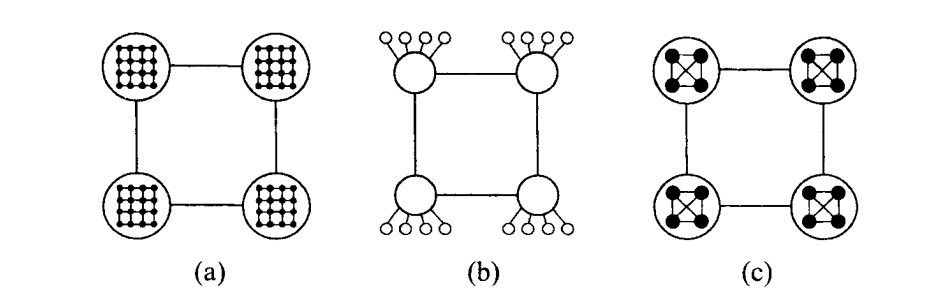
\includegraphics[scale=0.5]{hibridniModeli.png}
	\end{center}
	\caption{\dvareda{Primer nekih hibridnih modela: na baznom nivou su\\(a) ćelijski, (b) gospodar-sluga, (c) distribuirani model \cite{alba}}}
	\label{fig:hibridniModeli}
\end{figure}

U nastavku teksta će detaljnije biti opisani paralelni modeli algoritama evolucije.

\begin{enumerate}
    \item \textbf{Model sa nezavisnim pokretanjima}: \newline \indent \indent Ovaj model podrazumeva paralelno pokretanje istog sekvencijalnog algoritma bez interakcija između nezavisnih pokretanja. Ovaj krajnje jednostavan simultani metod je veoma koristan. Na primer, kada se želi više pokretanja algoritma za isti problem sa različitim inicijalnim vrednostima, prikupljajući na taj način statistike o problemu. Pošto je sama priroda genetskih algoritama stohastička, postojanje ovakvih statistika se smatra značajnim \cite{alba}.
    \newline
    Može se smatrati da je ovaj model specijalni slučaj distribuiranog modela gde ne postoje migracije. Ovako, rezultat distribuiranog izračunavanja je najbolje moguće rešenje iz nezavisnih izvršavanja \cite{alba}. 
    \item \textbf{Gospodar-sluga model}: \newline \indent Kod ovog modela master procesor izvršava glavnu petlju genetskog algoritma i šalje potrebne parametre slugama, koji koristeći te parametre izračunavaju funkciju evaluacije. Vrednosti ovih funkcija se potom vraćaju master procesoru \cite{alba}.
    \indent Pokazalo se da je ovaj model veoma efikasan kada je izračunavanje fitnesa veoma skupa operacija (u poređenju sa cenom komunikacije između master i sluga procesora).
    \item \textbf{Distribuirani model}: \newline \indent Nad svakom potpopulacijom se nezavisno izvršava genetski algoritam. Iako povremeno dolazi do migracija jedinki iz jedne subpopulacije u drugu, one su veći deo vremena izvršavanja međusobno izolovane. Distribuirani model zahteva postojanje \textit{planova migracija} koji uključuju postojanje sledećih parametara: \cite{alba}
    \begin{itemize}
        \item \textit{razmak između migracija} -- broj koraka u evoluciji u svakoj potpopulaciji između dve razmene, Migracije mogu da se događaju ili periodično ili sa određenom, unapred zadatom verovatnoćom $P_M$, za odluku u svakom koraku da li dolazi do migracije, ili ne,
        \item \textit{stopa migracije} -- koji broj jedinki će učestvovati u migraciji; može se izraziti u procentima celokupne populacije, ili kao apsolutna vrednost,
        \item \textit{odabir/zamena jedinki} -- kojim se biraju pojedinačne jedinke koje će biti zamenjene, kao i jedinke kojim se menjaju,
        \item \textit{topologija} -- definiše suseda za svaku subpopulaciju. Subpopulacija može svojim susedima da šalje, kao i da preuzima pojedinačne jedinke u procesu migracije.  
    \end{itemize}{}
\end{enumerate}{}

Svakodnevni razvoj mrežnih infrastruktura, softvera, internet servisa, kao i neprestano širenje mreža dovelo je do potrebe za novim algoritmima koji će zameniti tradicionalne koji su neefikasni kad su u pitanju problemi u industriji. Ta potreba za bržim rešenjima zadovoljena je upotrebnom metaheuristika u oblasti telekomunikacija, kao i paralelizacije, kojom bi te metaheuristike dodatno bile ubrzane. Jedan od glavnih problema u telekomunikacijama je problem Štajnerovog drveta (eng. \textit{Steiner Tree Problem}, STP), koji podrazumeva pronalaženje podstabla minimalne težine datog grafa uspostavljenih terminalnih čvorova. U radu \cite{fatta} predložen je gospodar-sluga paralelni GA kao konkretno rešenje ovog problema. Nakon toga je u radu \cite{martins} ovaj predlog proširen predstavljanjem hibridnog paralelnog modela koji kombinuje distribuirani GA i lokalnu pretragu koristeći specifične STP heuristike. Analiza efikasnosti pokazuje da distribuirani model postiže bolje vrednosti ubrzanja od gospodar-sluga modela jer koristi nekoliko tačaka sinhronizacije i na taj način može da se izvršava u okruženju računarskih mreža širokog pojasa \cite{alba}.

\subsection{Pristupi zasnovani na unapređenju rešenja}
\label{sec:ParalelizacijaJednog}

Osnovna ideja metaheuristika zasnovanih na unapređenju je započinjanje od jednog inicijalnog rešenja, koje se u većini koraka pretrage zamenjuje drugim rešenjem iz okruženja. Ovakve tehnike omogućavaju da se lokalna optimalna rešenja nađu brzo, ali stvaraju problem ako se zahteva globalno optimalno rešenje. Važno je napomenuti da tokom razmatranja kvaliteta u cilju zamene rešenja, na izbor može uticati i konkretna metoda koja je odabrana.
Na primeru metode simuliranog kaljenja, ako su određeni kriterijumi ove konkretne metode zadovoljeni, može se izabrati novo rešenje čija vrednost funkcije cilja nije bolja od vrednosti trenutne. Ovo takođe znači da nije izabrano rešenje koje ima najbolju vrednost funkcije cilja do koje se može dođi iz trenutnog rešenja, čimr se smanjuje verovatnoća konvergencije rešenja ka lokalnom optimumu koji nije i globalni \cite{talbi}.

Ovakve metode se nazivaju pretraživačko-orijentisane metode (eng. \textit{exploration-based}), jer se zalažu za pretraživanje prostora rešenja.
Metaheuristike za rešavanje optimizacionih problema se mogu 
posmatrati kao kretanje kroz prostor rešenja, prateći puteve nekog metoda pretrage.

Većina metaheuristika su sekvencijalne. Same po sebi imaju cilj da smanje vremensku složenost, ali uvek je moguće pribeći paralelizmu za još brža rešenja, mada paralelizam više doprinosi kvalitetu rešenja u ovom slučaju \cite{alba2}. U najpoznatije metode koje se zasnivaju na unapređenju jednog resenja, uz neke manje poznate poput pohlepne slučajne adaptivne pretrage (eng. \textit{Greedy Randomized Adaptive Search}, GRASP), spadaju:

\begin{itemize} 
\item simulirano kaljenje,
\item tabu pretraga,
\item iterativna lokalna pretraga,
\item metod promenljivih okolina.
\end{itemize}

U daljem tekstu je dat opšti algoritam za ove metode. Promenljiva 's' predstavlja niz izabranih rešenja određenih pretragom. Pre petlje se inicijalizuje početno rešenje metodom 'Generisi' i promenljiva 't', koja broji korake kretanja.
U petlji, koja se izvršava sve dok nije ispunjen kriterijum zaustavljanja pretrage, funkcijama 'IzaberiKorak', 'PrihvatiKorak' i 'PrimeniKorak' istražuje se prostor rešenja i prihvataju ona koja zadovoljavaju kriterijum vezan za konkretnu metodu koja se koristi.

\begin{algoritam}[H]
\SetAlgoLined
 $Generisi(s(0)$)\;
 $t := 0$\;
 \While{not kriterijumZaustavljanja(s(t))}{
  $s'(t) := IzaberiKorak(s(t))$\;
  \If{PrihvatiKorak(s'(t))}{
   $s(t) := PrimeniKorak(s'(t))$\;
   }
   $t := t+1$\;
 }
\caption{Sekvencijalni algoritam metaheuristike zasnovane na unapređenju jednog rešenja}
\end{algoritam}

Pretraga je iterativna i omogućava kretanje od jednog do drugog rešenja u prostoru rešenja. Pretraga počinje od jednog nasumičnog rešenja ili nekog dobijenog uz pomoć nekog drugog optimizacionog algoritma. U svakoj iteraciji trenutno rešenje je zamenjeno nekim drugim iz skupa susednih kandidata. Pretraga prestaje kad je dati uslov zadovoljen, kao npr. maksimalni broj pomeranja, nađeno rešenje je zadovoljavajućeg kvaliteta, algoritam ne pravi znatna poboljšanja tokom nekog određenog vremena \cite{alba2}.

Paralelizacija ovih algoritama se prvi put spominje u naučnim krugovima 1980. godine. Jačine procesora u to vreme su bile slabe tako da su gorenavedeni algoritmi u serijskom izvršavanju bili vremenski zahtevni čak i za manje probleme. Vremenom su procesori postajali sve jači, što je uticalo na rast zainteresovanosti i istraživanja ove oblasti. Razni nezavisni autori su davali slične predloge klasifikacije modela paralelizacije ovih algoritama, između kojih postoji mnogo preklapanja u ključnim idejama modela. Na slici \ref{fig:albaPodela} je dat vizuelni prikaz klasifikacije modela koje je predložio Enrike Alba, koji se najviše istakao u istraživanju ove teme \cite{alba}.

Najčešće predlagani modeli paralelizacije su:

\begin{enumerate}
\item \textbf {Model paralelizma podataka}: \newline \indent
Ideja ovog modela je podela podataka na delove između procesorskih jedinica.
Samim tim je i prostor rešenja podeljen.
Preduslov je da su podaci (prostor rešenja) razdvojivi.

\item \textbf {Model paralelizma kretanja}: \newline \indent
Na početku svake iteracije, program kopira trenutno rešenje između procesorskih jedinica. Informacije o vrednostima iz okoline se prikupljaju i prema njima
se bira sledeći kandidat/rešenje. Ovaj model
ne utiče na rešenje jer bi sekvencijalno izvršavanje
dalo iste rezultate samo u dužem vremenskom periodu.

\item \textbf {Model paralelizma višestrukog pokretanja}: \newline \indent
Najpopularnija metoda zbog lakoće korišćenja.
Algoritam se pokreće više puta istovremeno na različitim procesorskim jedinicama, sa različitim inicijalnim rešenjima, ili sa istim inicijalnim rešenjima, ali sa drugim parametrima. Ova metoda doprinosi boljem pokrivanju prostora rešenja.
Jedan od benefita ove metode je to što se može obezbediti
međusobna komunikacija između pokrenutih algoritama tokom njihovog izvršavanja,
korišćenjem memorije koje će deliti, i time pomoći drugim pokrenutim jedinicama ako su pre njih istražili neki deo prostora. 

\item \textbf {Model ubrzanog kretanja}: \newline \indent
Na početku svake iteracije, program koristi
paralelizaciju za izračunavanje funkcija cilja. Ovo je korisno ako funkcija može takođe biti paralelizovana pa se funkcija kvaliteta rešenja koji se posmatra u trenutnoj iteraciji može posmatrati kao agregacija
 parcijalnih funkcija.

\item \textbf {Hibridni model}: \newline \indent
Kombinovanje datih algoritama i modela paralelizma sa evolutivnim algoritmima koji su inherentno paralelni. Najčešće se koristi u kombinaciji sa modelom paralelizma višestrukog pokretanja gde se nad svakom jedinkom iz evolutivnog algoritma pokrene algoritam zasnovan na unapređenju jednog rešenja na odvojenim procesorskim jedinicama.
\end{enumerate}

Pokazalo se da je paralelizacija ovih metaheuristika veoma korisna kada je u pitanju rešavanje problema u oblasti telekomunikacija. Pouzdanost u telekomunikacijama odnosi se na mogućnost mreže da nesmetano funkcioniše kada dođe do kvara na nekom čvoru ili vezi. Pristup za povećavanje pouzdanosti u telekomunikacijskoj mreži sastoji se u ograničavanju broja grana na putanji između dva čvora -- postoji unapred uspostavljen skup čvorova i putevi između njih imaju najviše k grana.

Autori Riberio i Rozeti\cite{ribe} razvili su paralelni GRASP algoritam za ovaj problem kada je k = 2.
Faza konstrukcije GRASP-a koristi iterativni algoritam za određivanje najkraćeg puta u grafu, i to nasumičnim odabirom početnih i krajnjih čvorova sve dok svaka kombinacija parova nije razmotrena. Faza lokalne pretrage pokušava da poboljša rešenja eliminišući neke puteve i preračunavajući puteve koristeći modifikovane težine grana. Paralelni pristup koristi strategiju višestruke nezavisne pretrage dok se iteracije distribuirano izvršavaju na procesorima. Paralelizam omogućava linearno ubrzanje i dovodi do dostizanja većeg kvaliteta rešenja \cite{alba}.

\begin{figure}[h!]
	\begin{center}
		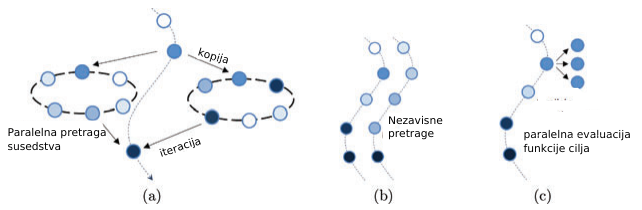
\includegraphics[scale=0.6]{albaPodela.png}
	\end{center}
	\caption{\dvareda{Modeli paralelizma prema Enrikeu Albi: (a) kretanje,\\(b) višestruko pokretanje, (c) ubrzano kretanje \cite{alba2}}}
	\label{fig:albaPodela}
\end{figure}

\section{Zaključak}
\label{sec:zakljucak}
Kako je i izloženo, paralelizacija je jedan od načina da se ubrza izvršavanje metaheuristika, a nekad i da se poboljša kvalitet rešenja. Paralelizacija ima i potencijal da se prilagodi problemima sa većim dimenzijama, kao i brojnim ograničenjima. Ipak, nije uvek sigurno da će paralelizacija, kao ni metaheuristika dati najbolje ili najbrže rešenje. Uz to, stalni razvoj tehnologije čini da izgleda kao da je potrebno mnogo znanja za pribegavanje parelelizaciji. Zato je, još uvek, ova oblast veliki izazov.

\newpage 

\addcontentsline{toc}{section}{Literatura}
\appendix
\bibliography{SM_14_ParalelizacijaMetaheuristickihAlgoritama_MirkovVasovicGolubovicHeldrih}
\bibliographystyle{unsrt}

\end{document}